% diagrams/english/flores.tex -- tres flores en una maceta, para "Read
% and colour": a la izquierda un tulipán, en el medio una margarita (los
% pétalos y el centro, aparte) y a la derecha una rosa; los tallos con
% sus hojas, y la maceta con su borde.
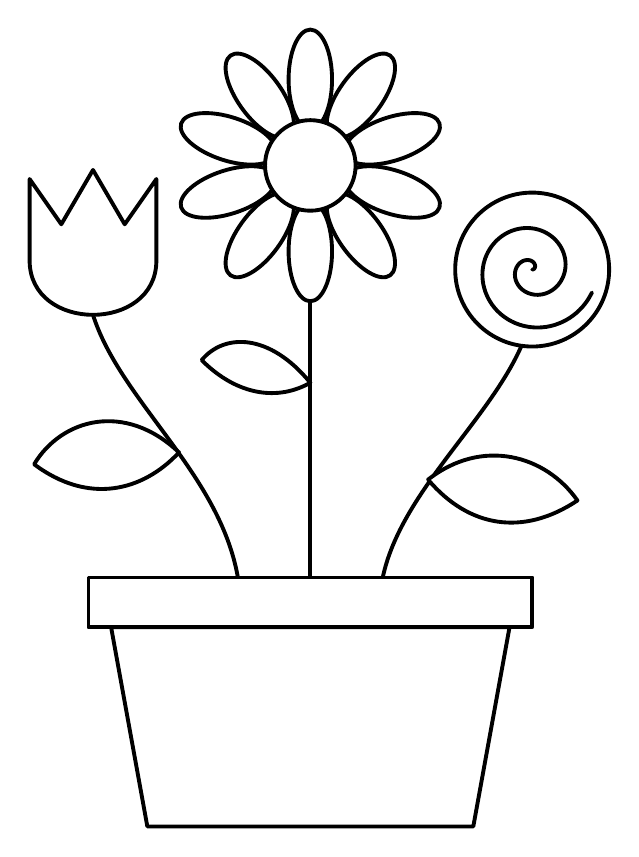
\begin{tikzpicture}[line width=1.4pt, line cap=round, line join=round, scale=1.15]
  % los tallos
  \draw (-0.8,2.75) .. controls (-1.0,3.9) and (-2.1,4.7) .. (-2.4,5.65);
  \draw (0,2.75) -- (0,6.3);
  \draw (0.8,2.75) .. controls (1.0,3.7) and (2.0,4.5) .. (2.35,5.35);
  % las hojas
  \filldraw[fill=white] (-1.45,4.13) .. controls (-2.05,4.7) and (-2.75,4.5) .. (-3.05,4.0)
    .. controls (-2.45,3.55) and (-1.85,3.7) .. cycle;
  \filldraw[fill=white] (0,4.9) .. controls (-0.45,5.45) and (-0.95,5.45) .. (-1.2,5.15)
    .. controls (-0.8,4.75) and (-0.35,4.7) .. cycle;
  \filldraw[fill=white] (1.3,3.83) .. controls (1.9,4.3) and (2.6,4.1) .. (2.95,3.6)
    .. controls (2.35,3.2) and (1.75,3.3) .. cycle;
  % la maceta y su borde
  \filldraw[fill=white] (-1.8,0) -- (-2.2,2.2) -- (2.2,2.2) -- (1.8,0) -- cycle;
  \filldraw[fill=white] (-2.45,2.2) rectangle (2.45,2.75);
  % el tulipán, a la izquierda
  \filldraw[fill=white] (-3.1,6.25) .. controls (-3.1,5.45) and (-1.7,5.45) .. (-1.7,6.25)
    -- (-1.7,7.15) -- (-2.05,6.65) -- (-2.4,7.25) -- (-2.75,6.65) -- (-3.1,7.15) -- cycle;
  % la margarita, en el medio: los pétalos y, encima, el centro
  \foreach \a in {0,36,...,324} {
    \filldraw[fill=white, rotate around={\a:(0,7.3)}] (0,8.25) ellipse (0.24 and 0.55);
  }
  \filldraw[fill=white] (0,7.3) circle (0.5);
  % la rosa, a la derecha: el contorno y la espiral de dentro
  \filldraw[fill=white] (2.45,6.15) circle (0.85);
  \draw plot[domain=0:12.2, samples=90, smooth, variable=\t]
    ({2.45 + 0.058*\t*cos(\t r)}, {6.15 + 0.058*\t*sin(\t r)});
\end{tikzpicture}
